\documentclass[12pt]{article}
\usepackage[12pt]{moresize}

\usepackage{amsmath}
\usepackage{amssymb}

\usepackage{graphicx}
\usepackage{subcaption}

\usepackage{algorithm}
\usepackage{algpseudocode}
\usepackage{alltt}

\usepackage{multicol}

\usepackage[margin=1in]{geometry}

%\usepackage{hyperref}
%\usepackage[latin1]{inputenc}
%\usepackage{listings}
%\usepackage{scrextend}
%\usepackage{changepage} %Adjustwidth


\newenvironment{PTMono}{\fontfamily{PTMono-TLF}\selectfont}{\par}


\title{ComS 363\\Homework 1}
\author{Sean Gordon}
%\date{09/09/2019}

\begin{document}
\maketitle


\hrulefill \\



\noindent 1)

\begin{multicols}{2}
\begin{PTMono} \footnotesize

\noindent CREATE TABLE Artist (\\
\indent Artist\_Name VARCHAR(50),\\
\indent   Birthplace VARCHAR(50),\\
\indent   DOB DATE,\\
\indent   Art\_Style VARCHAR(50),\\
  
 PRIMARY KEY (Artist\_Name)\\
);\\\\



\noindent CREATE TABLE Art (\\
\indent   Artist\_Name VARCHAR(50),\\
\indent   Year\_Made DATE,\\
\indent   Art\_Title VARCHAR(50),\\
\indent   Art\_Type VARCHAR(50),\\
\indent   Price INT,\\
  
 PRIMARY KEY (Art\_Title),\\
\indent   FOREIGN KEY (Artist\_Name) \\
\indent \indent  REFERENCES Artist\\
);\\\\



\noindent CREATE TABLE Art\_Group (\\
\indent Group\_Name VARCHAR(50),\\
\indent  Art\_Title VARCHAR(50),\\
  
 PRIMARY KEY (Group\_Name),\\
\indent  FOREIGN KEY (Art\_Title) \\
  \indent \indent REFERENCES Art\\
);\\


\columnbreak


\noindent CREATE TABLE Customer (\\
\indent   Cust\_Name VARCHAR(50),\\
\indent   Address VARCHAR(50),\\
\indent   Total\_Spent INT,\\
  
  PRIMARY KEY (Cust\_Name)\\
);\\



\noindent CREATE TABLE Likes (\\
\indent   Cust\_Name VARCHAR(50),\\
\indent   Art\_Title VARCHAR(50),\\
\indent   Group\_Name VARCHAR(50),\\
  
  FOREIGN KEY (Cust\_Name) \\
\indent \indent REFERENCES Customer\\
\indent   FOREIGN KEY (Art\_Title) \\
\indent \indent REFERENCES Art\\
\indent   FOREIGN KEY (Group\_Name) \\
\indent \indent REFERENCES Art\_Group\\
);\\


\end{PTMono}
\end{multicols}


\pagebreak


\begin{figure}[h!]
  \centering
  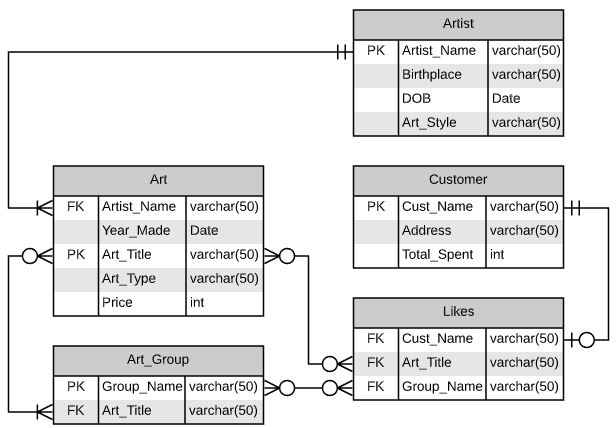
\includegraphics[scale=1]{Pt1_ERDiagram.JPG}
\end{figure}





\hrulefill
\pagebreak





\noindent 2)

\begin{multicols}{2}
\begin{PTMono} \footnotesize

\noindent CREATE TABLE Student (\\
\indent  First\_Name VARCHAR(50),\\
\indent  Last\_Name VARCHAR(50),\\
\indent  Student\_ID INT,\\
\indent  SSN INT,\\
\indent  Curr\_Address VARCHAR(50),\\
\indent  Phone VARCHAR(11),\\
\indent  Perm\_Address VARCHAR(50),\\
\indent  Perm\_Phone VARCHAR(11),\\
\indent  DOB DATE,\\
\indent  Gender VARCHAR(50),\\

PRIMARY KEY (Student\_ID)\\
);\\\\



\noindent CREATE TABLE Department (\\
\indent Name VARCHAR(50),\\
\indent Dep\_Code INT,\\
\indent Office\_Phone VARCHAR(11),\\
\indent College VARCHAR(50),\\

  PRIMARY KEY (Dep\_Code)\\
);\\\\



\noindent CREATE TABLE Course (\\
\indent  Name VARCHAR(50),\\
\indent  Description VARCHAR(50),\\
\indent  Course\_ID INT,\\
\indent  Credit\_Hours INT,\\
\indent  Course\_Level INT,\\
\indent  Dep\_Code INT,\\

  PRIMARY KEY (Course\_ID),\\
\indent   FOREIGN KEY (Dep\_Code) \\
\indent \indent REFERENCES Department\\
);\\\\



\noindent CREATE TABLE Degree (\\
\indent  Degree\_Level INT,\\
\indent  Degree\_Name VARCHAR(50),\\
\indent  Dep\_Code INT,\\

  PRIMARY KEY (Degree\_Name),\\
\indent   FOREIGN KEY (Dep\_Code) \\
\indent \indent REFERENCES Department\\
);\\\\



\columnbreak


\noindent CREATE TABLE Major (\\
\indent  Student\_ID INT,\\
\indent  Degree\_Name VARCHAR(50),\\

FOREIGN KEY (Student\_ID) \\
\indent \indent REFERENCES Student\\
\indent   FOREIGN KEY (Degree\_Name) \\
\indent \indent REFERENCES Degree\\
);\\\\



\noindent CREATE TABLE Minor (\\
\indent  Student\_ID INT,\\
\indent  Degree\_Name VARCHAR(50),\\

FOREIGN KEY (Student\_ID) \\
\indent \indent REFERENCES Student\\
\indent   FOREIGN KEY (Degree\_Name) \\
\indent \indent REFERENCES Degree\\
);\\\\



\noindent CREATE TABLE Registered (\\
\indent  Student\_ID INT,\\
\indent  Course\_ID INT,\\

FOREIGN KEY (Student\_ID) \\
\indent \indent REFERENCES Student\\
\indent   FOREIGN KEY (Course\_ID) \\
\indent \indent REFERENCES Course\\
);\\

\end{PTMono}
\end{multicols}


\pagebreak


\begin{figure}[h!]
  \centering
  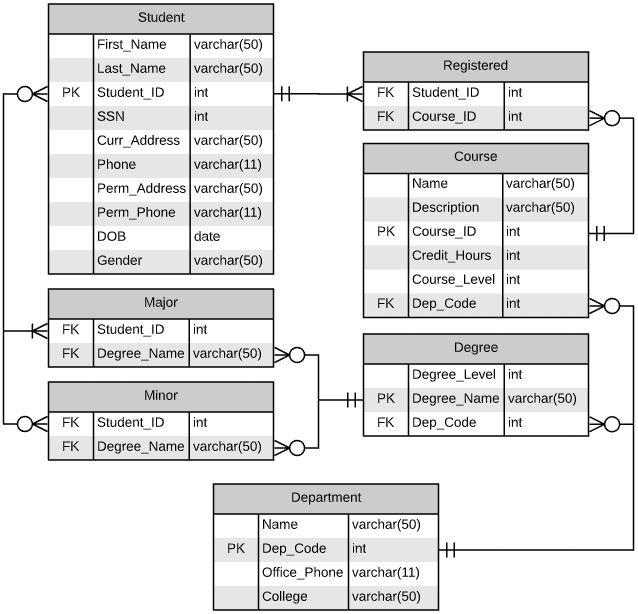
\includegraphics[scale=1]{Pt2_ERDiagram.JPG}
\end{figure}



\end{document}
















